% Pacotes e configurações padrão do estilo ``article''\
% -------------------------------------
\documentclass[a4paper,11pt]{article}
% Layout
% ------------------------------------------------------------------------------
%     Gráficos e layout ----------------------------------------------------------------------

\ifx\pdfmatch\undefined
\else
    \usepackage[T1]{fontenc}
    \usepackage[utf8]{inputenc}
\fi
% xetex:
\ifx\XeTeXinterchartoks\undefined
\else
    \usepackage{fontspec}
    \defaultfontfeatures{Ligatures=TeX}
\fi
% luatex:
\ifx\directlua\undefined
\else
    \usepackage{fontspec}
\fi
% End engine-specific settings

%      Fonte --------------------------------------------------------------------------------
%\usepackage{lmodern}
\usepackage{times}
%     Pacotes adicionados -------------------------------------------------------------------
\usepackage{ae}
%     Língua e hifenização ------------------------------------------------------------------
\usepackage[portuguese]{babel}
\usepackage{hyphenat}
%      Outros --------------------------------------------------------------------------------
\usepackage{hyperref} % Permite Links personalisados usando hyperref
\usepackage{fancyhdr}
\usepackage{sectsty}
\usepackage{float}   % Gerencia melhor o posicionamento das figuras e tabelas
%\usepackage{graphicx}
\usepackage[pdftex]{color,graphicx}
\usepackage{hyperref}
\usepackage{enumerate} % Permite alterar Layout do enumerate
%\usepackage{pdflscape}  % Permite alterar a orientação da pagina para Paisagem
%\usepackage{ifthen}  % Permite usar condicionais ifelse
%\usepackage[table]{xcolor} % Permite alterar as cores das células de uma tabela
\usepackage{amsmath,amssymb} % Ambiente para uso de elementos matemáticos
\usepackage{caption}
\usepackage{subcaption} % permite o uso de multiplas figuras com legenda (ambiente subfigure)
\usepackage{minted} % Ambiente minted para colorir código de programas
\usepackage{natbib} % Para referencia bibliográfica
\usepackage{url}    % Referência de links na internet
%\usepackage{listings} % pacote para apresentar código de programação
\usepackage{indentfirst}  % Para indentar o primeiro parágrafo de cada seção
\usepackage{titling}  % Permite Montar uma página de titulo própria

% Layout do documento ------------------------------------------------------------------------
%     Bordas e tamanho da página ------------------------------------------------------------
\usepackage{geometry} 
 \geometry{ % Padrõa ABNT para relatórios
 a4paper,
 left=30mm,
 right=20mm,
 top=30mm,
 bottom=20mm
 }
%     Cabeçalho e Rodapé ---------------------------------------------------------------
\pagestyle{fancy}
  \lhead{}
  \chead{}
  \rhead{}
  \lfoot{}
  \cfoot{}
  \rfoot{\thepage}
%     Númeração ------------------------------------------------------------------------
  \pagenumbering{arabic}
%     Retas do cabeçalho e rodapé ------------------------------------------------------
  \renewcommand{\headrulewidth}{0.5pt}
  \renewcommand{\footrulewidth}{0.5pt}
%     Tamanho da letra de seções e derivadas --------------------------------------------
  \sectionfont{\normalsize}
  \subsectionfont{\small}
%     Hiperlinks ------------------------------------------------------------------------
  \hypersetup{
                  colorlinks,
                  citecolor=black,
                  filecolor=black,
                  linkcolor=black,
                  urlcolor=black
                  }
%     Definições do pdf ----------------------------------------------------------------------
\hypersetup{
    unicode=false,          % non-Latin characters in Acrobat’s bookmarks
    pdftoolbar=true,        % show Acrobat’s toolbar?
    pdfmenubar=true,        % show Acrobat’s menu?
    pdffitwindow=false,     % window fit to page when opened
    pdfstartview={FitH},    % fits the width of the page to the window    
    pdfauthor={Rafael Lima},     % author
    pdfnewwindow=true      % links in new window
}
%     Outros ----------------------------------------------------------------------------
      %\renewcommand{\thesection}{(\alph{section})} % muda o estilo de númeração das sections
      % alterando a formatação dos numeradores de lista de itens
      \renewcommand\theenumi{\arabic{enumi}}
      \renewcommand\labelenumi{(\textit{\theenumi})}
	  \renewcommand\theenumii{\arabic{enumii}}
	  \renewcommand\labelenumii{(\textit{\theenumi.\theenumii})}
      
% ---------------------------------------------------------------------------------------


%\usepackage{circuitikz}
\usepackage[clean]{svg}

\title{Proposta de projeto - Controle discreto de um motor DC} % Define o título do Relatório
\author{Rafael Lima}

% Definições Auxiliares ( Macros próprias )
% ------------------------------------------------------------------------------
%\input{relat_aux.tex} % Arquivo com minhas macros
% ----------------------------------~>ø<~---------------------------------------
\begin{document}
% Capa e Índice ----------------------------------------------------------------
%--------------------------------------------------- Capa --------------------------------------------
%\newpage
\begin{figure}[h!]
\centering

\includegraphics[scale=0.9]{img/simb_unb.png}
\label{fig:unb}
\end{figure}

\begin{center}
{\LARGE Universidade de Brasília}\\
Departamento de Engenharia Elétrica\\
Professor: Henrique Cezar Ferreira\\
Disciplina: Controle Digital\\
\end{center}


\vspace{0.18\textheight}

\begin{center}
    \Huge \textbf{\\\thetitle \\}
\end{center}

\vspace*{\fill} % Completa espaço em branco e empurra o resto para o final da página

% Tabela com os nome das pessoas do grupo

\begin{table}[H]
    \begin{tabular}{ll}
        % Nome      & Matrícula
        Rafael Lima & 10/0131093 \\
        Leonardo Cardoso Botelho & 11/0154151 \\
    \end{tabular}
\end{table}

\vspace{0.5cm}

\begin{center}
    \textbf{Brasília\\
    \the\year} % Coloca o Ano atual
\end{center}

\thispagestyle{empty} % Retira o cabeçalho e o rodapé da página

% ------------------------------------------------- Índice -------------------------------------------
\newpage
\tableofcontents
\newpage
% ----------------------------------------------------------------------------------------------------

 % Capa para UnB
% Conteúdo ---------------------------------------------------------------------

\section{Introdução}

O presente trabalho discorre sobre o desenvolvimento de um servo mecanismo a partir de técnicas de controle discreto com base em uma planta composta por um motor DC (motor de corrente contínua), um sistema de redução e um sensor encoder de maneira a permitir o controle da posição a partir de um sinal de referência. O conjunto de peças foi retirada de um equipamento antigo que havia sido descartado. Para implementação do controle, além da planta foi utilizado um Arduino UNO e uma módulo com uma ponte H para o controle de potência conforme mostrado na figura \ref{fig:dispositivos}.

\begin{figure}[H]
    \centering
    \begin{subfigure}[b]{0.32\linewidth}
        \centering
        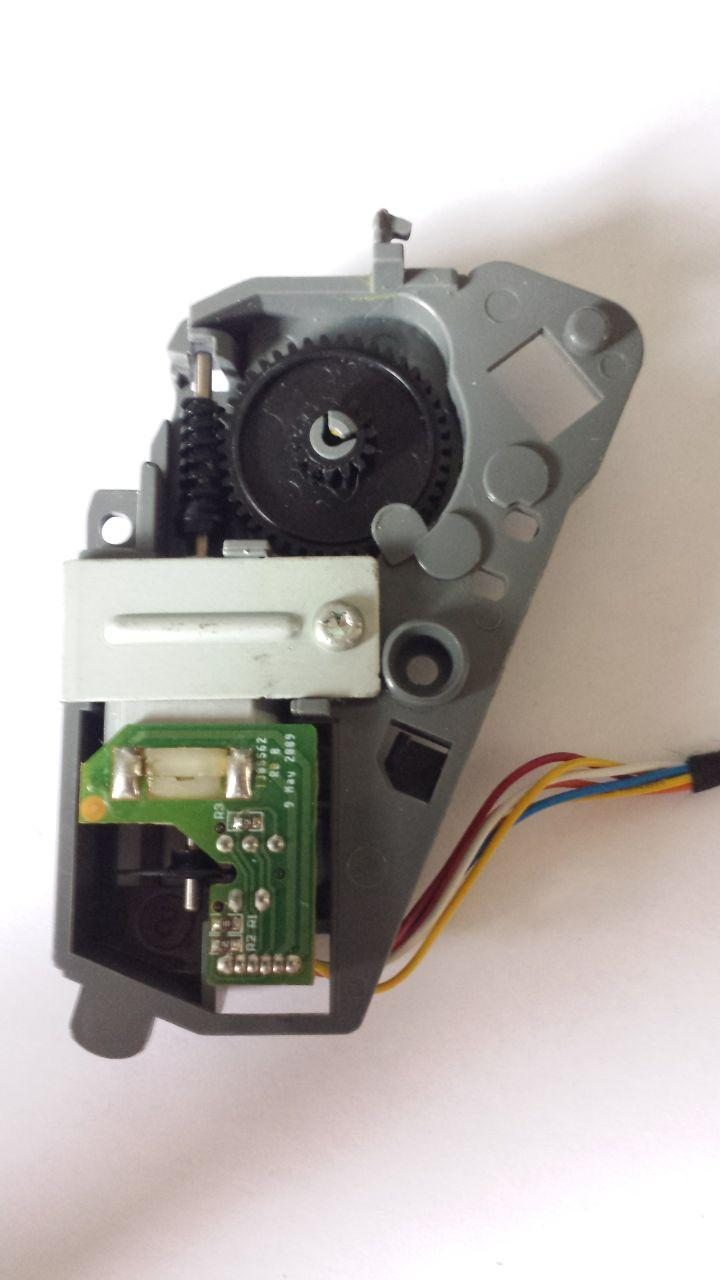
\includegraphics[width=0.8\linewidth]{src/tex/img/servomotor.jpg}
        \caption{Conjunto Motor DC + Encoder}
    \end{subfigure}
    \hfill
    \begin{subfigure}[b]{0.32\linewidth}
        \centering
        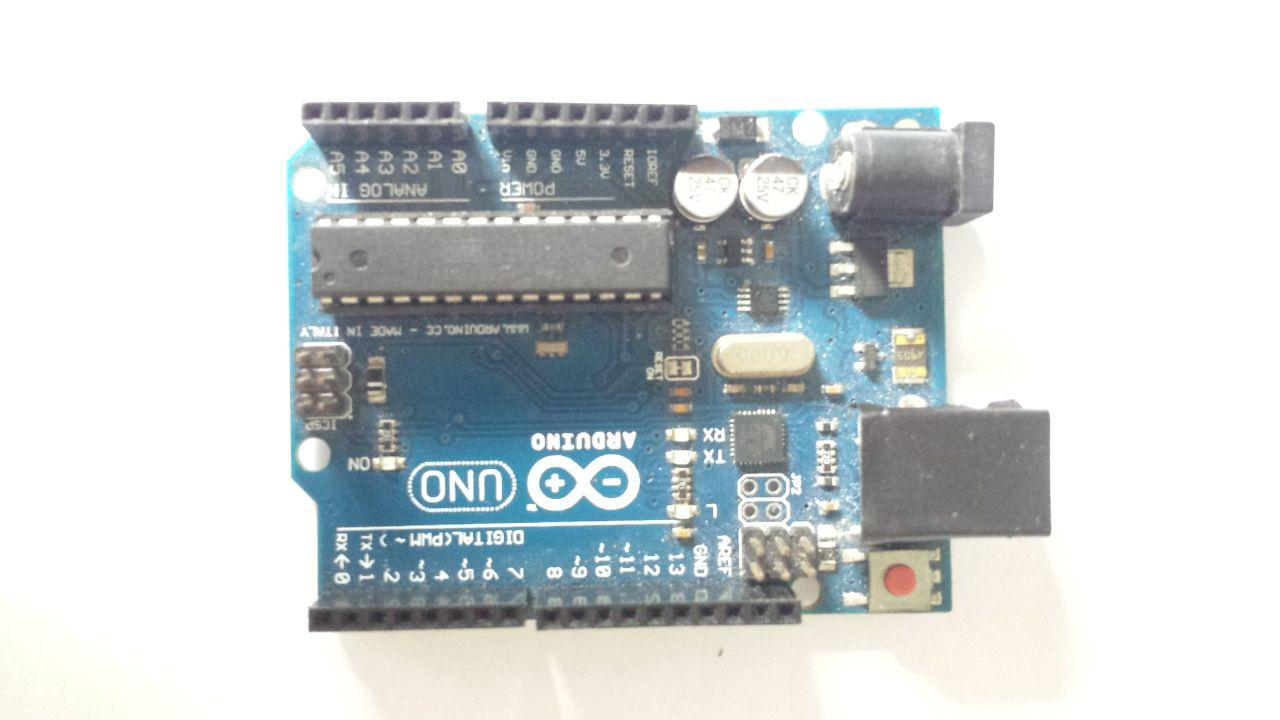
\includegraphics[height=0.9\linewidth, angle=90]{src/tex/img/arduinoUNO.jpg}
        \caption{Arduino UNO}
    \end{subfigure}
    \hfill
    \begin{subfigure}[b]{0.32\linewidth}
        \centering
        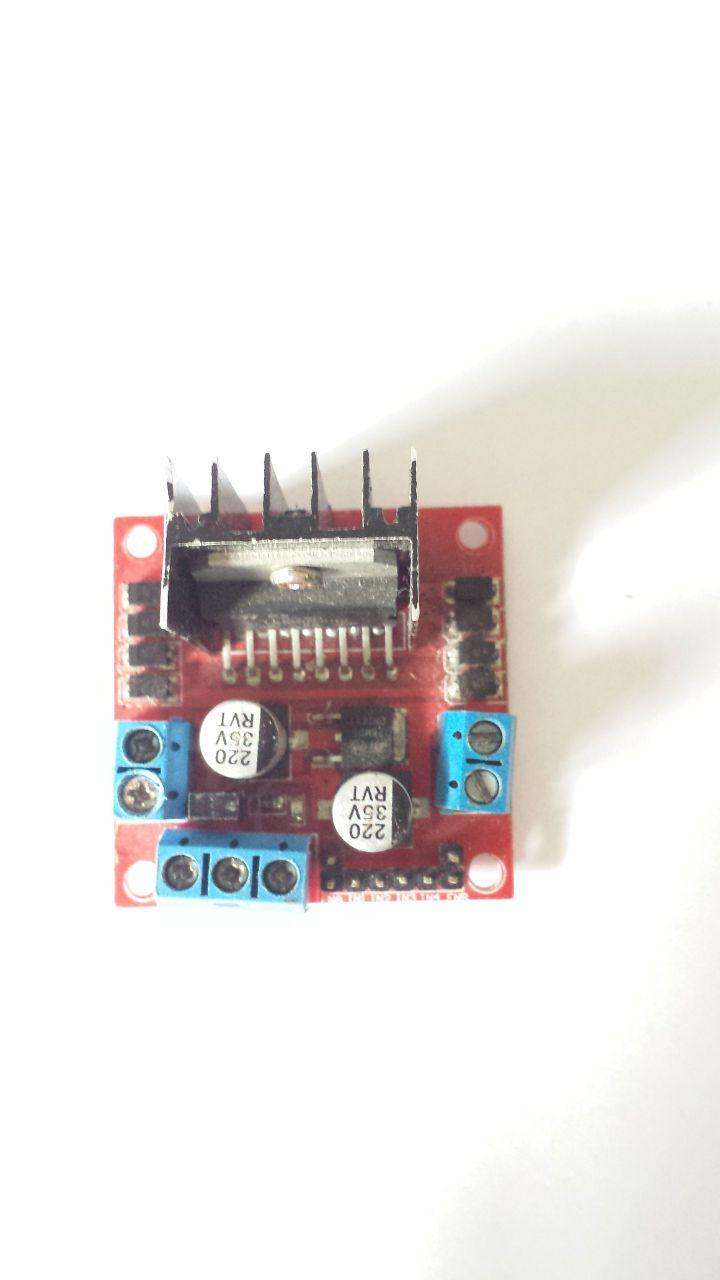
\includegraphics[width=0.9\linewidth]{src/tex/img/ponteH.jpg}
        \caption{Ponte H}
    \end{subfigure}
    \caption{Peças para proposta da planta}
    \label{fig:dispositivos}
\end{figure}

\subsection{Justificativa}

Sistemas de posicionamento utilizando motores de corrente contínua está presente nos mais variados equipamentos presentes nos dia de hoje. Isso se dá pois eles possuem bom custo benefício, 

Sua complexidade é razoável para o contexto da disciplina de Controle de Digital pois temos nesse sistema pelo menos dois atrasos nos elementos de atuação e sensoreamento. A caixa de redução por sua vez também insere um aspecto interessante ao processo, visto os efeitos de histerese e zona morta.

Do ponto de vista didático, esse sistema possui bons elementos a serem compreendidos no contexto da disciplina de Controle Digital. Podemos destacar as etapas de modelagem, discretização da planta, alocação de polos no domínio Z, projeto em LGR no domínio discreto de um controlador, identificação de sistema e implementação em uma planta real.

Por fim, o controle digital pressupõe um sistema computacional para sua execução, podendo ser operado por um microcontrolador disponível a custo acessível comercialmente. Isso torna esse projeto relevante no contexto das aplicações que utilizam motores de corrente contínua.

\subsection{Objetivos}

Este projeto têm seguintes objetivos:

 \begin{enumerate}
   \item Obter modelo da planta no domínio da frequência (Motor DC em conjunto com caixa de redução);
   \item Obter modelo do sensor no domínio da frequência;
   \item Obter modelos discreto da planta em conjunto com o sensor
   \item Desenvolver modelo em \textit{Simulink} para o projeto
   \item Obter controlado descrito através de equações de diferenças;
   \item Implementação e Validação do controlador em teste no sistema real;
 \end{enumerate}

\subsection{Metodologia de Projeto}

Para o desenvolvimento do projeto foi feito a partir das etapas relatadas a seguir. Primeiramente foi feito uma revisão bibliográfica e modelagem da planta e avaliação em ambiente de simulação. Num segunda fase foi ajustado o modelo encontrado para o planta real.

\begin{itemize}
    \item Estudo Planta em Simulação
    \begin{enumerate}
        \item Revisão Bibliográfica para busca do modelo de um servo motor na literatura
        \item Simulação do modelo
        \item Implementação do controle em simulação
    \end{enumerate}
    \item Estudo Planta Real
    \begin{enumerate}
        \item Simulação da planta no \textit{Tinkercad}
        \item Identificação de Parâmetro da Planta
        \item Simulação da planta a partir do modelo identificado
        \item Implementação do controle em simulação
        \item Implementação do controle na planta
    \end{enumerate}
\end{itemize}

\section{Desenvolvimento}

O desenvolvimento foi feitas em 3 fases: implementação em hardware, caracterização do sistema e projeto do controlador. Primeiramente foi feito um estudo e caracterização de cada um dos componentes, depois foram feitos vários testes visando a identificação do modelo da planta bem como suas propriedades do ponto de vista de controle e por fim foi desenvolvido um controlador a partir dos dados obtidos experimentalmente que pudesse permitir o funcionamento do sistema a partir dos requisitos desejados.

\subsection{Implementação em Hardware}

Para o projeto de um sistema de controle é necessário garantir alguns requisitos básicos do ponto de vista de acionamento, sensoriamento e temporização. Primeiramente é necessário que os atuadores e os sensores deve possuir um faixa de operação compatível com a dinâmica esperada do sistema. Além disto deve ser observado também o tempo necessário para a ação de controle como forma de garantir uma amostragem com período constante, permitindo assim o uso da teoria de controle desenvolvida ao longo da disciplina.

Como efeito, em virtude da natureza dos componentes escolhidos, foi necessário implementar algumas funcionalidades do zero. Em particular um tempo maior foi necessário na leitura do deslocamento angular a partir do sensor óptico em no acionamento do motor conjunto com o Arduino. Este estudo foi implementado primeiramente no \textit{Tinkercad} e posteriormente foi feito diretamente na planta.

\subsubsection{Simulação no Tinkercad}

Como forma de prevenir danos as peças, foi utilizado o \textit{Tinkercad} para simulação do sistema e como uma plataforma de estudos a respeito do comportamento do motor DC em conjunto com o encoder incremental. O \textit{Tinkercad} foi escolhido por sua simplicidade de uso e facilidade de integração do circuito diretamente com a programação do Arduino.

\begin{figure}[H]
    \centering
    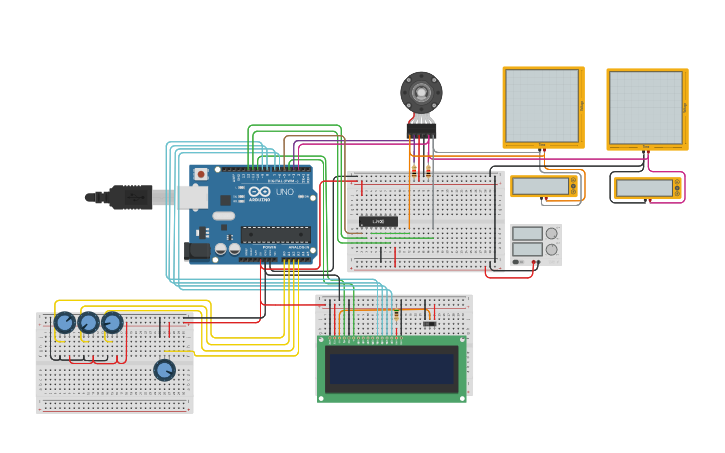
\includegraphics[width=\linewidth]{src/tex/img/pid_tinkercad.png}
    \caption{Diagrama Sistema implementado no Tinkercad}
    \label{fig:pid_tinkercad}
\end{figure}

Desta forma foi possível avaliar os algoritmos usados para a contagem de passo pelo encoder em conjunto com o acionamento do motor, cálculo do PID e detecção de sentido de rotação. Conforme ilustrado pela figura \ref{fig:pid_tinkercad}, foram utilizados potenciômetros para um ajuste manual e grosseiro dos ganhos do PID. Também foi adotado um display para mostrar os ganhos adotados. Com isto foi possível chegar a uma combinação de ganhos que permitia o motor alcançar o valor da referência ou ao menos parar após um tempo de movimento.

Uma atenção maior foi dada a como obter e condicionar os dados do encoder e como definir uma estrutura mínima do código para acondicionar tanto o acionamento como a leitura dos sensores dentro do período escolhido. Com isto foi possível gerar alguns gráficos iniciais da variação da posição ao longo do tempo. Porém dado as limitações da plataforma, principalmente nos modelos adotados para o motor e para comportamento das portas e ações do Arduíno não foi possível adotar nenhuma forma de identificação dos parâmetros.

O maior problema encontrado foi que o tempo real gasto pelo funções do Arduino não era obedecido pela simulação e com isto não dava para verificar qual a frequência máxima que poderia ser usada para amostragem. Assim, concluído o estudo preliminar passamos para experimentos feitos diretamente na planta real.

\subsubsection{Temporização}

Como o estilo de controlador adotado pressupõe uma amostragem fixa, foi necessário adotar um controle de temporização estrito como forma de garantir que tanto o acionamento como a leitura do encoder seria feita dentro do tempo adequado. A leitura de cada passo do encoder é feita através de interrupção e a frequência de acionamento é feita a partir da comparação do valor de tempo para o instante atual com temporizadores internos. Para avaliar o tempo gasto em um conjunto de instruções foi adota uma estratégia similar registrando os valores intermediários e enviando para a serial, uma vez que não tinha disponível nenhum osciloscópio ou equipamento de medida externo para esta avaliação.

\subsubsection{Leitura Encoder}

O encoder presente na planta escolhida é sistema ótico e incremental e com isto foi necessário adicionar ao código no Arduíno a contagem de passos a detecção de sentido de rotação. O sinal do encoder é composto por duas ondas quadradas defasadas em 90 graus. Desta forma, o deslocamento absoluto pode ser obtido através da contagem dos pulsos e o sentido de rotação pela comparação do dois sinais.

% TODO Adicionar Ilustração do sinal do encoder

Como esta variação é relativamente rápida, o sinal de borda de subida do encoder foi associado a uma interrupção no processador. Como efeito a cada vez que é detectado um pulso, o processamento é interrompido e uma função para contagem e detecção da direção é chamada. Desta forma é possível manter o algoritmo de controle em paralelo com a leitura do encoder.

A partir da captura de dados movendo-se manualmente o eixo do motor foi detectado a presença de bastante ruído na leitura. Foi percebido nos primeiros experimentos que contador acabava sendo incrementado ainda que o motor estivesse parado. Para reduzir o ruído algumas medidas foram adotadas: primeiro o sinal de alimentação do encoder foi separado do sinal de alimentação da ponte H, foi adotado um cabo com par trançado como forma de reduzir a interferência devido ao ruído introduzido com o acionamento do motor, a fonte de alimentação do motor e do arduino também foi separada. Com estas medidas, o ruído reduziu bastante.

\subsubsection{Acionamento Motor}

O acionamento do motor foi feito através de uma ponte H. Um fator que introduz não linearidade ao sistema é a presença de uma zona morta correspondente ao mínimo de tensão necessária para fazer o motor girar partindo do repouso. Além disto o sistema possui uma limitação de tensão máxima que é capaz de fornecer, o que também impõe um limite a região linear para controle do motor.

\subsection{Caracterização Sistema}

\begin{figure}[H]
    \centering
    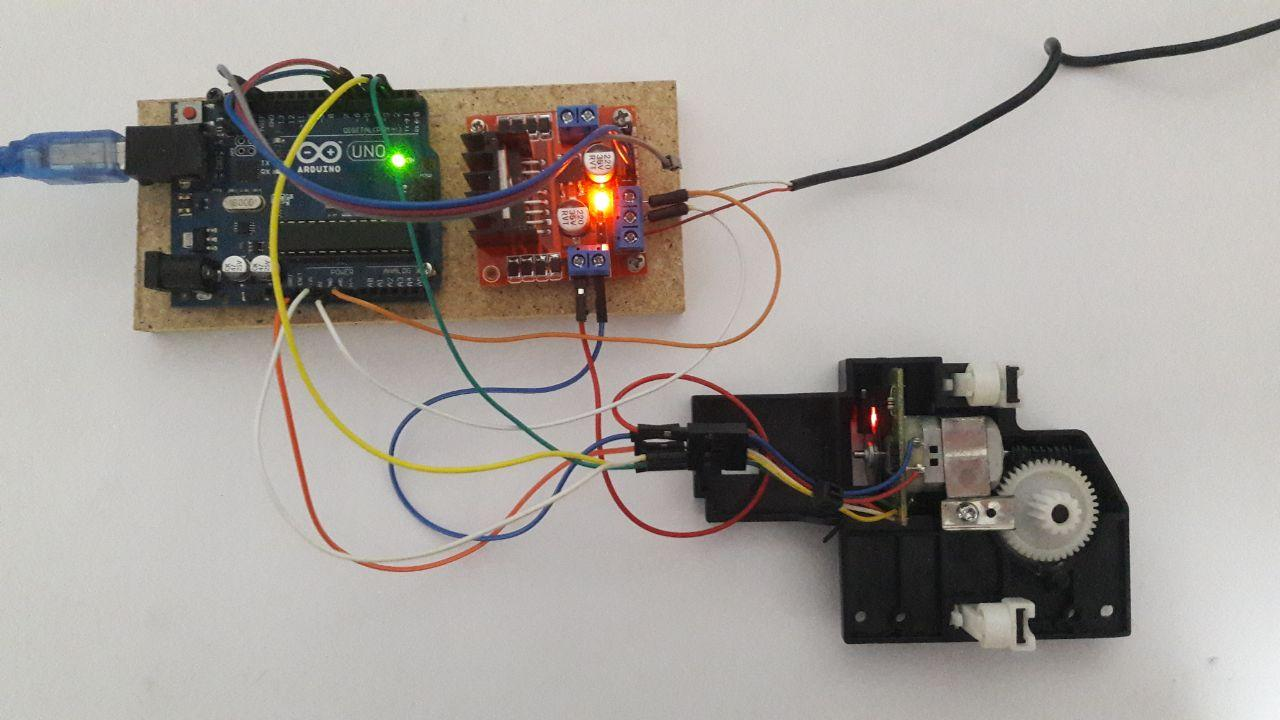
\includegraphics[width=\linewidth]{src/tex/img/full_system.jpg}
    \caption{Planta Montada}
    \label{fig:pid_tinkercad}
\end{figure}

\begin{figure}[H]
    \centering
    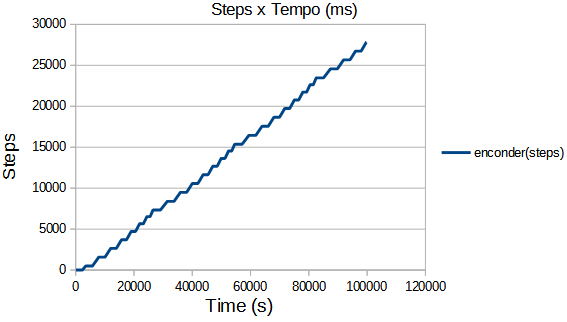
\includegraphics[width=\linewidth]{src/tex/img/grafico_steps.PNG}
    \caption{Steps x tempo (ms)}
    \label{fig:steps}
\end{figure}

\begin{figure}[H]
    \centering
    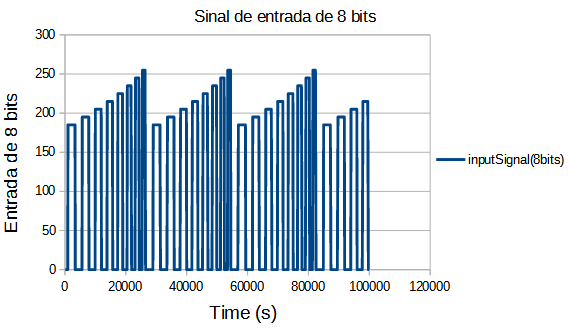
\includegraphics[width=\linewidth]{src/tex/img/sinal_8_bits.PNG} 
    \caption{Sinal de 8 bits}
    \label{fig:sinal8bits}
\end{figure}

\begin{figure}[H]
    \centering
    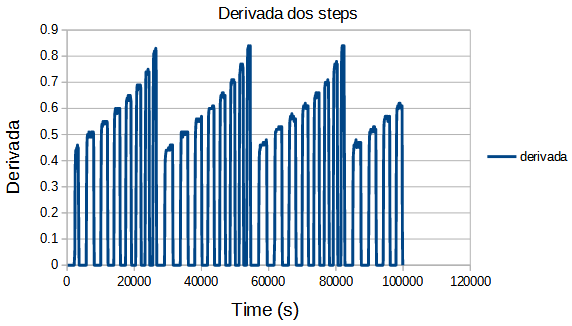
\includegraphics[width=\linewidth]{src/tex/img/derivada_steps.PNG} 
    \caption{Derivada do sinal}
    \label{fig:sinal8bits}
\end{figure}

\subsubsection{Região Não Linear}

Idealmente o comportamento poderia ser representado através de um modelo linear para todas as condições de operação, No entanto, na prática devido as características do hardware, temos uma região de operação a qual o modelo pode ser utilizado delimitada por uma região inferior e superior.

Para o motor começar a se mover é preciso fornecer um mínimo de energia. Esta quantidade varia de acordo com as características eletromecânicas do motor. Em particular para o motor utilizado, a faixa de operação é de 3V a 6V, sendo 3V o mínimo para fazer o motor girar e 6V uma tensão máxima para não danificar.

A conversão do sinal de controle do Arduino em um sinal de potência foi feita através uma ponte H em conjunto com um sinal PWM. Como efeito, a tensão de alimentação da fonte utilizada para o motor foi amostrada usando 8 bits. Desta forma, chegar ao valor teórico correspondente a zona morta do motor para uma alimentação de 5V basta 

$$
D_{min} = \frac{3V}{V_{fonte}}(2^8 -1) = \frac{3*255}{5} = 153
$$

Para obter este valor experimentalmente foi feito um programa aplicando um sinal de entrada de dente de serra (em anexo). Isto é, o valor de referência passado para a tensão do motor foi gradualmente aumentado e em seguida gradualmente reduzido de forma periódica. Os valores obtidos foram registrados a partir do Matlab através da conexão Serial com o Arduino.

Mesmo que frequência interna do Arduino seja próximo de $14 MHz$, as operações de comunicação via Serial são bastante dispendiosas. Por conta disto, o menor período conseguido experimentalmente a qual é mantida um a operação com ciclo em tempo contante foi de $60ms$. Foi escolhido então uma período de $100ms$ de forma a permitir uma margem segura de folga de tempo para todas as operações. Para períodos menores que este valor, o tempo gasto com a comunicação serial, cálculos e as interrupções do encoder acabava sendo maior que o período de amostragem fixo e as garantias de funcionamento em tempo real eram perdidas.

%% TODO Adicionar Gráfico Leitura Arduino onda Dente de Serra

\subsubsection{Identificação de Parâmetros}

Uma vez definido uma região linear de operação foi adotado o procedimento de identificação do sistema. Pelas especificação do fabricante temos

\begin{table}[H]
    $$
    \begin{array}{ccc}
         \hline
         V_i\ [V] & \dot{\theta}\ [RPM] & \dot{\theta}\ [Hz]\\
         \hline
         3 & 3000 & 50 \\
         6 & 6000 & 60 \\
         \hline
    \end{array}
    $$
    \caption{Velocidade de operação sem carga}
    \label{tab:dcmotor_speed}
\end{table}

De forma que poderíamos adotar como uma aproximação razoável do comportamento dinâmico do motor como uma função de transferência de primeira ordem na forma

\begin{equation}
    G_m(s) = \frac{\beta}{\alpha s + 1}
\end{equation}

Neste sistema temos apenas a medida da posição através do encoder. Este processo é feito através do conjunto de várias etapas, incluindo amostragem através da contagem do pulsos e a discretização referente ao instante de contabilização da leitura do sensor. No entanto, dado a grande diferença entre o tempo gasto neste processo com o tempo gasto na comunicação serial, podemos aproximar a dinâmica do sistema de medição de posição como um ganho fixo.

Feito as devidas considerações, a planta sem controlador pode ser representada da seguinte forma

%% TODO Acrescentar diagrama de blocos do sistema em malha aberta ( ZOH + Planta de 1 ordem + integrador  + ganho)

Aplicando a transformada Z podemos representar o sistema em tempo discreto pela seguinte função:

\begin{equation}\label{eq:gz_general}
    G(z) = \frac{Y(z)}{U(z)} = \frac{\beta_1 z + \beta_2}{z^2 + \alpha_1 z + \alpha_2}
\end{equation}

Do que podemos observar que a discretização traz como efeitos tanto o deslocamento dos polos, como também a inclusão de um zero na planta.

A partir da função \ref{eq:gz_general} podemos obter a representação do sistema a partir de equação de diferenças como:
% $$
% Y z^2
% $$

\begin{equation}\label{eq:gz_general}
  Y[k+2] = -Y[k+1]\alpha_1 - Y[k]\alpha_2 + U[k+1]\beta_1 + U[k]\beta_2
\end{equation}

Tomando um conjunto maior de dados podemos reescrever a equação na forma matricial como

\begin{equation}\label{eq:gz_general}
  Y[k+2] = 
  \left( \begin{array}{cccc}
  -Y[k+1] & -Y[k] & U[k+1] & U[k]
  \end{array} \right)
  \left(\begin{array}{c}
    \alpha_1\\ \alpha_2 \\ \beta_1 \\ \beta_2
  \end{array}\right)
\end{equation}

A partir do qual podemos relacionar o sinal de saída com o sinal de entrada do sistema e obter os parâmetros $\alpha_1$,$\alpha_2$,$\beta_1$ e $\beta_2$ por regressão linear. Para obter uma melhor caracterização foi gerado um sinal formado por pulsos de tamanhos e durações variadas diretamente no Arduino. % Conforme mostrado na figura \ref{}

%% TODO Adicionar Gráfico Leitura Arduino onda pulsos

Os dados do tempo, leitura do encoder e sinal de referência foram então enviados para o computador através de comunicação serial e com auxílio do Matlab (código em anexo) foi obtido a seguinte função de transferência:

\begin{equation}
G(z) = \frac{Y(z)}{U(z)} = \frac{0.19422\,z-0.092392}{z^2-1.6576\,z+0.65762}
\label{transfdisc}
\end{equation}

Onde o período de amostragem é de $T = 100 ms$, o tempo é dado em $ms$ e o sinal de entrada e saída em $bits$.

\subsection{Projeto do controlador}

A planta escolhida para esse trabalho é um dispositivo tipicamente utilizado para posicionamento de cartuchos de impressoras e scanners. Esse equipamentos não tem requisitos tão rígidos quanto velocidade como servos motores de aeromodelos e possuem baixa tolerância para grandes valores de sobressinal. 

\subsubsection{Definição Requisitos}

O desempenho do controlador será algo dentro dos limites físicos dos dispositivos envolvidos. No que inclui, a taxa de variação da posição angular não pode ser maior que $10Hz$, a precisão está bastante limitada as taxas de amostragem de 8 bits do Arduino e quantidade de buracos do disco do encoder. Tendo isto em mente foi definido como requisitos para o sistema:

\begin{itemize}
   \item Overshoot <= 16 \%;
   \item Tempo de assentamento para entrada degrau: 1 s;
 \end{itemize}

\subsection{Primeira proposta de controlador}

O primeiro controlador tem seu projeto feito pelo LGR (Lugar Geométrico das Raízes). Analisa-se o LGR da planta discretizada no plano imaginário Z. Para o requisito de overshoot, procura-se um ponto no LGR em que o fator de amortecimento esteja entre o intervalo de 0.5 e 0.7, visto a seguinte relação em \ref{UP}:

\begin{equation}
\zeta=\frac{-\ln \left(P O\% / 100\right)}{\sqrt{\pi^{2}+\ln ^{2}\left(P O\% / 100\right)}}
\label{UP}
\end{equation}

Nesse primeiro momento procura-se atender apenas um dos objetivos, tendo como objetivo final dessa etapa encontrar um ganho dentro do LGR da planta que atenda o requisito. 

Em momento posterior, analisa-se a resposta ao degrau em malha fechada do sistema para observar se o requisito de tempo de assentamento também foi alcançado utilizando apenas essa proposta. 

As etapas desta análise seguem na sequência a seguir:

\begin{enumerate}
   \item Dispor pólos e zeros da planta no plano imaginário;
   \item Obter o LGR da planta no espaço Z;
   \item Delimitar conjunto de pontos no plano imaginário que corresponde a fator de amortecimento de 0.7;
   \item Determinar ponto de intersecção do LGR com a linha do conjunto de dados de fator de amortecimento;
 \end{enumerate}

Utilizando-se a função \textit{rlocus} do Matlab (Função que gera o lugar da Raízes de uma função de transferência) e a função \textit{zgrid} (que plota a área do plano Z no plano imaginário), presentes no Matlab, temos na figura \ref{fig:lgr} o LGR da função de transferência da planta discretizada em \ref{transfdisc}:

\begin{figure}[H]
    \centering
    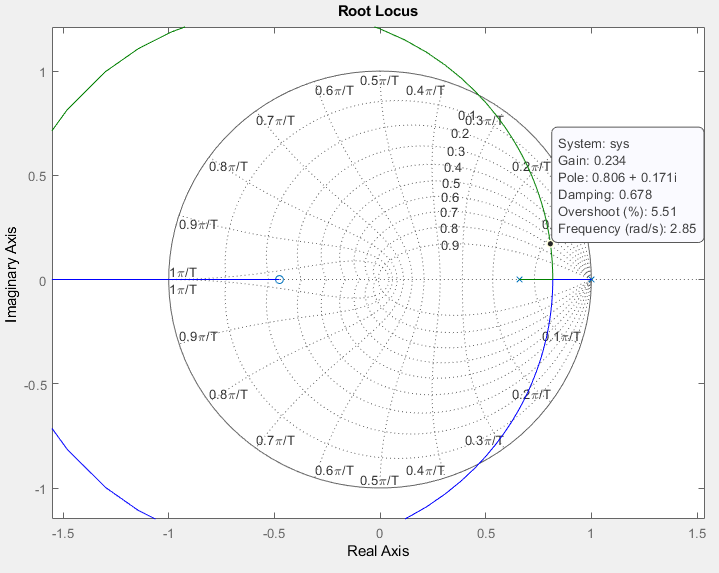
\includegraphics[width=\linewidth]{src/tex/img/rlocus.PNG}
    \caption{LGR da planta}
    \label{fig:lgr}
\end{figure}

Observa-se que o ganho para a obtenção do comportamento deseja do sistema é de $0.234$. Para validação desse resultado, simulou-se o sistema em malha fechado no Simulink com segue na figura \ref{fig:controle1}:

\begin{figure}[H]
    \centering
    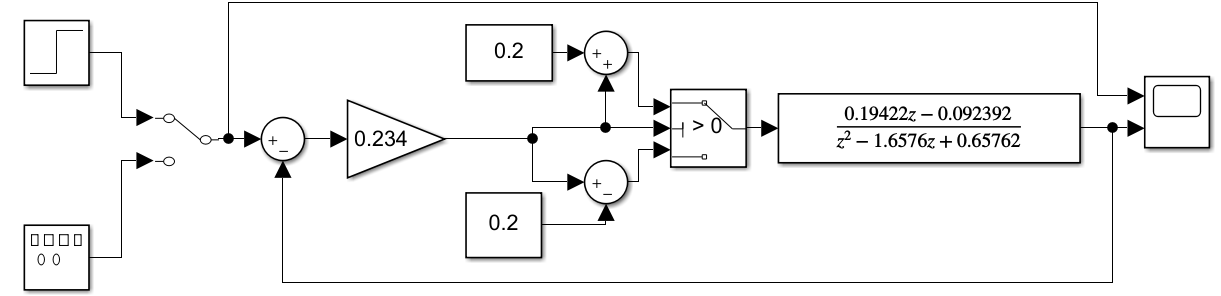
\includegraphics[width=\linewidth]{src/tex/img/controle_1.PNG}
    \caption{Diagrama da proposta 1 de controle}
    \label{fig:controle1}
\end{figure}

Os resultados obtidos estão dispostos a seguir nas figuras \ref{fig:saidactrl1} e \ref{fig:saidactrl1up}: 

\begin{figure}[H]
    \centering
    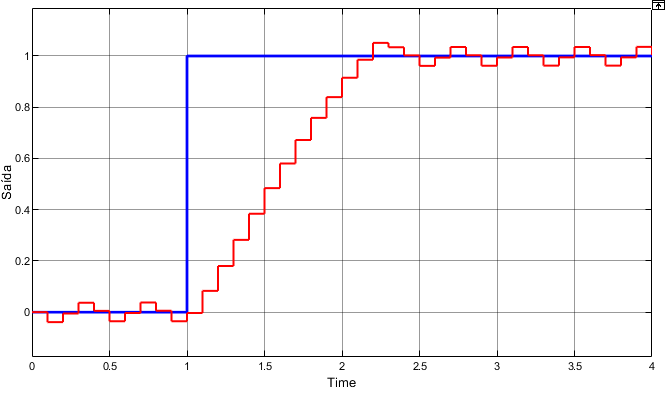
\includegraphics[width=\linewidth]{src/tex/img/saida_controle_1.png}
    \caption{Gráfico da saída da proposta 1 de controle}
    \label{fig:saidactrl1}
\end{figure}

Observa-se que o requisito de \textit{overshoot} foi alcançado. Na gráfico da figura \ref{fig:saidactrl1up} foi aumentado a escala do gráfico a fim de ser mais preciso quanto a essa análise. O \textit{overshoot} é aproximadamente de 5 \% com valores abaixo desse valor para o trecho em que o sinal já está estabilizado em 1.

\begin{figure}[H]
    \centering
    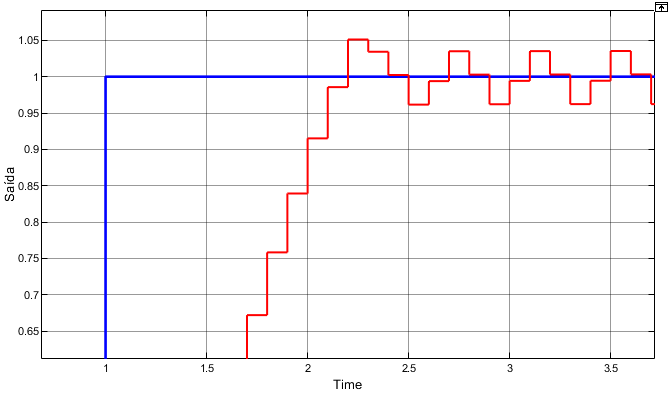
\includegraphics[width=\linewidth]{src/tex/img/saida_controle1_up.PNG}
    \caption{Aumento de escala para observação do \textit{overshoot} da proposta 1 de controle}
    \label{fig:saidactrl1up}
\end{figure}

A implementação em arduino do primeiro controlador segue na figura \ref{fig:resultadoctrl1}, em que foi utilizado um ganho de 0.25:

\begin{figure}[H]
    \centering
    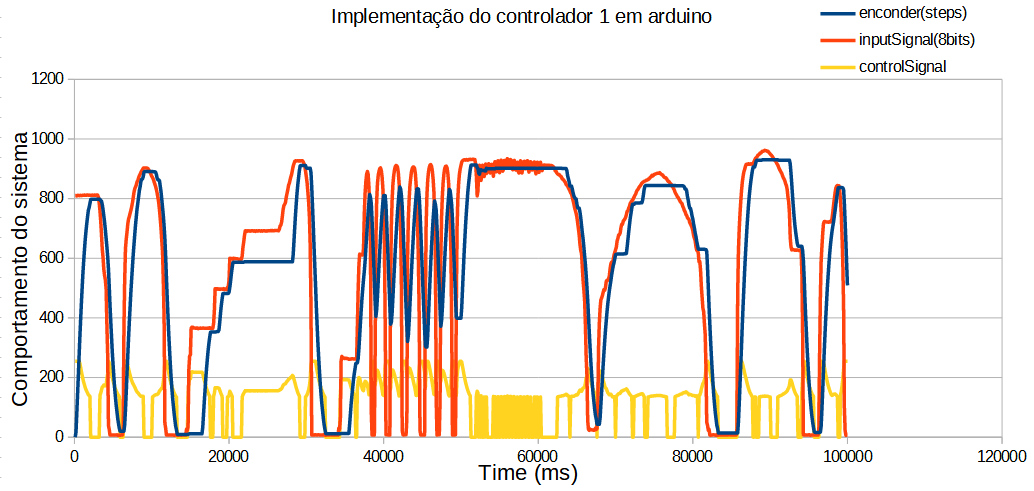
\includegraphics[width=\linewidth]{src/tex/img/resultado_controle_1_implem.PNG}
    \caption{Implementação em arduino do controlador 1}
    \label{fig:resultadoctrl1}
\end{figure}

 Entretanto, o tempo de assentamento é maior que 2 segundos, mais que o dobro do tempo de assentamento do requisito de projeto. Por esse motivo, propõe-se um segundo tipo de proposta de projeto. 

\subsection{Segunda proposta de controlador}

Nessa abordagem iremos utilizar o Diagrama de Bode. O objetivo é atender os dois requisitos realizando um compensador em avanço. Para isso, iremos realizar a transformada inversa de Z sobre a função de transferência discretizada, obtendo sua versão no domínio da frequência, como se segue em \ref{equacao_s}:

\begin{equation}
G(s) = \frac{0.5011(s+70.0259)}{(s+0.00058419)(s+4.19042)}
\label{equacao_s}
\end{equation}

Utiliza-se a estratégia de anular o polo de $4.19042$ da planta e adicionar um outro polo. A escolha do novo polo irá seguir a relação \ref{assentamento_eq}:

\begin{equation}
\zeta \omega_{n}=\frac{4}{T_{s}}
\label{assentamento_eq}
\end{equation}



Como se quer tempo de assentamento de 1 segundo, utiliza-se um fator de amortecimento menor sem deixar de se observar \textit{overshoot}. A escolha então será de fator de amortecimento de $0.5$. Tem-se então que a frequência natural para o caso é de \textbf{8 radianos por segundos}. O controlador tem a seguinte lei do formação \ref{novogc}:

\begin{equation}
G_{c}(s)=\frac{s+4.19042}{s+8}
\label{novogc}
\end{equation}

Plota-se então o Diagrama de BODE da planta para realizar a compensação de ganho devido ao avanço do novo controlador. Analisa-se que em próximo ao polo que é anulado na planta, o ganho é de $3.46\ dB$.

\begin{figure}[H]
    \centering
    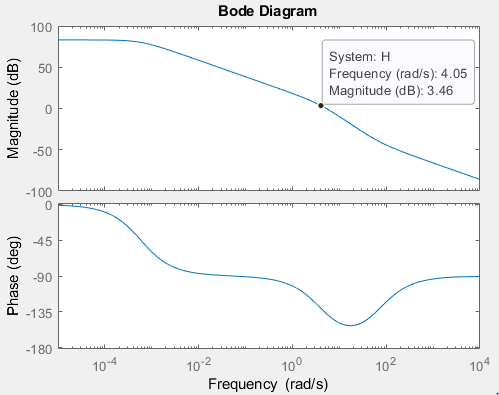
\includegraphics[width=\linewidth]{src/tex/img/bode.PNG}
    \caption{Diagrama da primeira proposta de controle}
    \label{fig:lgr}
\end{figure}

O controlador final fica então com a seguinte configuração (\ref{novogcz}):

\begin{equation}
G_{c}(z)=3.46\frac{s - 0.7116}{z - 0.4493}
\label{novogcz}
\end{equation}

Implementa-se então o controlador em Simulink a fim de avaliar o alcance dos requisitos, como segue na figura \ref{fig:projetoavanco}:

\begin{figure}[H]
    \centering
    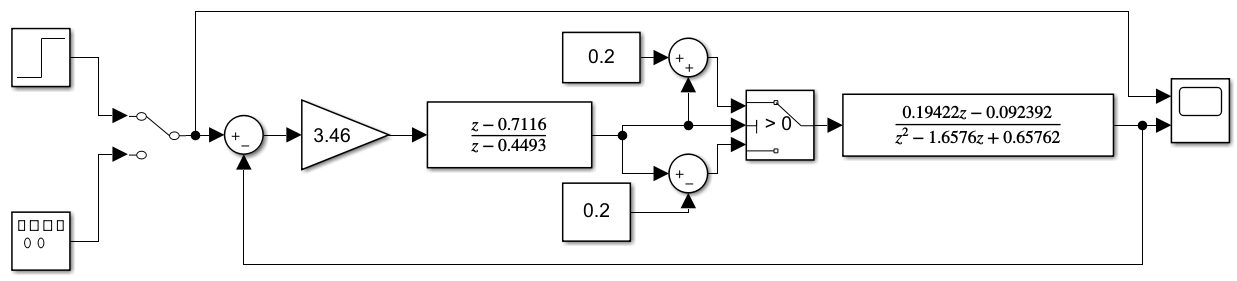
\includegraphics[width=\linewidth]{src/tex/img/controle_2.PNG}
    \caption{Diagrama da segunda proposta de controle}
    \label{fig:projetoavanco}
\end{figure}

Observa-se na figura \ref{fig:degrauavanco} que o requisito tempo de assentamento de 1 segundo é alcançado.

\begin{figure}[H]
    \centering
    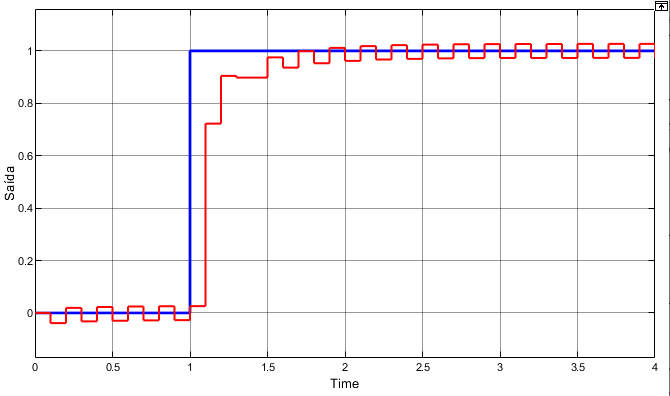
\includegraphics[width=\linewidth]{src/tex/img/saida_controle_2.png}
    \caption{Resposta ao degrau da segunda proposta de controle}
    \label{fig:degrauavanco}
\end{figure}

O \textit{overshoot} por sua vez fica abaixo de $5$ \%, e esse requisito também é resolvido.

\begin{figure}[H]
    \centering
    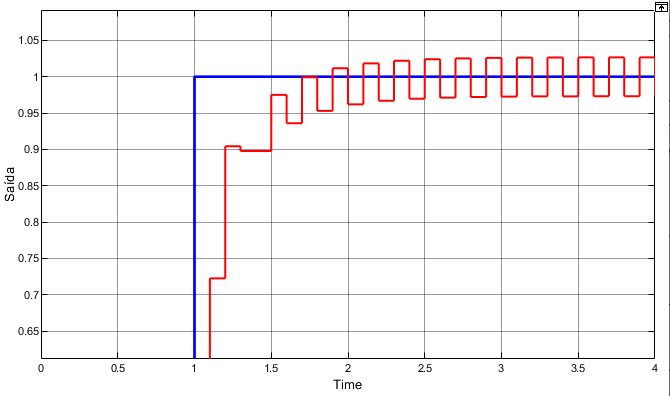
\includegraphics[width=\linewidth]{src/tex/img/saida_controle_2_up.PNG}
    \caption{Overshoot da segunda proposta de controle}
    \label{fig:lgr}
\end{figure}

Por fim, realizou-se um teste de stress no sistema com um sinal square de amplitude 1, o que seria semelhante ao carro do cartucho de um impressora se deslocando durante o processo de impressão.

\begin{figure}[H]
    \centering
    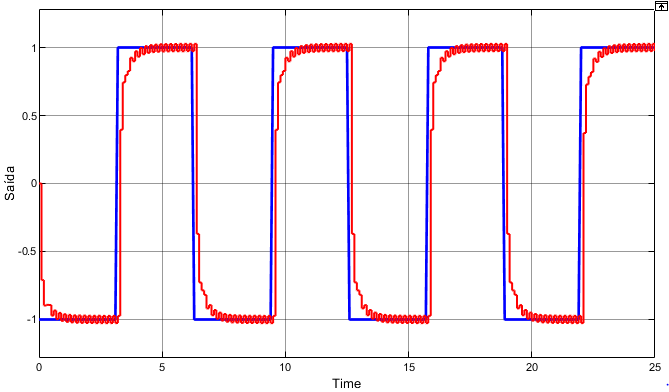
\includegraphics[width=\linewidth]{src/tex/img/teste_square.PNG}
    \caption{Resposta a squares}
    \label{fig:lgr}
\end{figure}

A função de transferência do caminho direto do sistema fica com o seguinte formato (\ref{caminhodireto}):

\begin{equation}
G(z)=(\frac{0.19422\,z-0.092392}{z^2-1.6576\,z+0.65762}) . (3.46\frac{z - 0.7116}{z - 0.4493})
\label{caminhodireto}
\end{equation}

Desenvolvendo-se algebricamente obtêm-se (\ref{caminhodiretodes}):

\begin{equation}
G(z)= \frac{Y(z)}{U(z)} = \frac{0.672001 z^{2}-0.797872 z+0.227482}{z^{3}-2.1069 z^{2}+1.40238 z-0.295469}
\label{caminhodiretodes}
\end{equation}

Por fim, a equação das diferenças do sistema é descrita em \ref{equacaodasdiferencas}:

\begin{equation}
\begin{split}
y[k]=0.672001 \cdot x[k-1]-0.797872 \cdot x[k-2]+0.227482 \cdot x[k-3] \\-2.1069 \cdot y[k-1]+1.40238 \cdot y[k-2]-0.295469 \cdot y[k-3]
\end{split}
\label{equacaodasdiferencas}
\end{equation}

A equação das diferenças é uma descrição do sistema adequada a ser utilizada em microcontroladores digitais.

\section{Conclusão}

A implementação de um sistema de controle de posição a partir de Arduino trouxe vários desafios. Preparar um hardware e garantir as mínimas condições de operação em tempo real para os controladores acabou tomando mais tempo que o previsto. Durante o processo alguns motores foram danificados e também houve perda de um encoder, porém tal representou uma excelente oportunidade de aprendizado tanto em como lidar com as características de cada dispositivo usado como também permitir uma compreensão melhor da teoria de controle.

Como abordagem principal, tanto na escolha do tema dos métodos utilizados foi buscado a todo momento a integração dos conhecimentos desenvolvidos da teoria de controle de sistema a tempo discreto em conjunto os campos de programação de microcontroladores, instrumentação digital e programação em tempo real. Esta abordagem trouxe seus ônus por acrescentar etapas no projeto além da simulação pura de um sistema físico idealizado, mas contribuiu bastante no melhor entendimento do impacto das características físicas e tipos de ruídos associados de cada parte no sistema de controle.

%% TODO Comentar sobre os resultados do controlador

A partir do estudo feito, foi possível projetar um controlador que atendesse os requisitos propostos tanto para o sistema real como simulado. Com as simplificações feitas na planta, reduzindo o frequência da dinâmica do controlador e da planta foi possível simplificar bastante o projeto final, de modo que um ganho proporcional foi o suficiente para atender os requisitos mínimos de desempenho. Em continuidade a este estudo, margens mais rígidas de desempenho podem ser testadas como forma de permitir o estudo de controladores mais complexos.

Embora não apresentado aqui, o estudo feito ao longo deste projeto permitiu verificar experimentalmente de forma qualitativa o comportamento da planta em malha fechada para diversos valores de ganho. Tendo sido possível perceber as regiões com comportamento amortecido, oscilação amortecida e instabilidade. O que contribuiu bastante para a consolidação dos conhecimentos desenvolvidos na matéria.

% ------------------------------------------------------------------------------
\newpage
% Referências
\addcontentsline{toc}{section}{Referências} % Adiciona linha no índice
\bibliographystyle{abbrv} % Define Estilo e gera bibliografia
\bibliography{references} % Adiciona Arquivo com Referências

% Acrescentadas no arquivo references.bib
% para usa-las no texto basta usar \citep{}
% para citar sem usar no texto basta usar \nocite{}
%\nocite{sympy}
%\nocite{pythontex}
\nocite{matlabcontrol}
\nocite{matlabsymbolic}
\nocite{ogata2010modern}

% ------------------------------------------------------------------------------
%\newpage
\section*{Anexos}
\addcontentsline{toc}{section}{Anexos} % Adiciona linha no indice
%\subsection*{Python}

%Para os cálculos e demonstrações foi utilizado o pacote \textit{Python}\TeX\ \cite{pythontex} para o \LaTeX\ em conjunto da bibliteca \textit{sympy}\cite{sympy}. Segue o script completo em python:

%\inputminted[xleftmargin=15pt,linenos,frame=single,framesep=5pt,breaklines=true]{python}{../python/exsim6.py}

%\newpage
\subsection*{Matlab}

\subsubsection*{Parte 1}
Para o desenho dos gráficos e simulações foi utilizado o \textit{Matlab} em conjunto das toolbox \textit{Control System}\cite{matlabcontrol} e \textit{Symbolic Math}\cite{matlabsymbolic}. Segue o código referente usado

\inputminted[xleftmargin=15pt,linenos,frame=single,framesep=5pt,breaklines=true]{matlab}{../matlab/project.m}

\newpage
\subsubsection*{Leitura dados Arduino}
\inputminted[xleftmargin=15pt,linenos,frame=single,framesep=5pt,breaklines=true]{matlab}{../matlab/plotArduino.m}

\newpage
\subsubsection*{Identificação de Parâmetros}
\inputminted[xleftmargin=15pt,linenos,frame=single,framesep=5pt,breaklines=true]{matlab}{../matlab/identification.m}

\newpage
\subsection*{Arduino}
Dado as limitações do Arduino foram produzidos diferentes códigos como forma de avaliar o funcionamento de cada componente de hardware isoladamente.

\subsubsection*{Teste Encoder}
Para avaliar o funcionamento do encoder foi usado o seguinte código
\inputminted[xleftmargin=15pt,linenos,frame=single,framesep=5pt,breaklines=true]{c++}{../arduino/test_enconder/test_enconder.ino}

\newpage
\subsubsection*{Teste Motor}
Para avaliar o funcionamento do motor foi usado o seguinte código
\inputminted[xleftmargin=15pt,linenos,frame=single,framesep=5pt,breaklines=true]{c++}{../arduino/test_dcmotor/test_dcmotor.ino}

\newpage
\subsubsection*{Teste Motor}
O código usado para caracterização da zona morta do sistema e avaliação do funcionamento conjunto do motor com o encoder foi usado o seguinte:
\inputminted[xleftmargin=15pt,linenos,frame=single,framesep=5pt,breaklines=true]{c++}{../arduino/test_dcmotor_characterization/test_dcmotor_characterization.ino}

\newpage
\subsubsection*{Identificação da planta}
O código usado para identificação dos parâmetros do planta:
\inputminted[xleftmargin=15pt,linenos,frame=single,framesep=5pt,breaklines=true]{c++}{../arduino/test_dcmotor_pulses/test_dcmotor_pulses.ino}

\newpage
\subsubsection*{Controle}
Para implementação do controlador foi usado o seguinte código
\inputminted[xleftmargin=15pt,linenos,frame=single,framesep=5pt,breaklines=true]{c++}{../arduino/pid_control/pid_control.ino}

% https://www.usinainfo.com.br/drivers-para-motores/driver-ponte-h-ou-motor-de-passo-l298-2302.html
% ------------------------------------------------------------------------------
\end{document}
